
\documentclass[dvipdfmx]{beamer}
\AtBeginShipoutFirst{\special{pdf:tounicode EUC-UCS2}}

\usetheme{Madrid}
\usecolortheme{default}
\setbeamerfont{frametitle}{size=\large,series=\bfseries}
\setbeamertemplate{navigation symbols}{}
\setbeamertemplate{footline}[frame number]
\setbeamertemplate{items}[circle]
\setbeamertemplate{section in toc}[circle]
\setbeamertemplate{blocks}[rounded][shadow=true]

\definecolor{character}{RGB}{0,0,0} %文字
\definecolor{background}{RGB}{245,245,245} %背景
\setbeamercolor{normal text}{bg=background, fg=character}

\definecolor{mathFormula}{RGB}{53,121,53} %数式
\setbeamercolor{math text}{fg=mathFormula}

\definecolor{alertColor}{RGB}{255,75,75} %alert
\setbeamercolor{alerted text}{fg=alertColor}

\definecolor{blockAlertColor}{RGB}{0,0,0} %alertblock内の文字
\setbeamercolor{block body alerted}{fg=blockAlertColor}

\definecolor{headColor}{RGB}{52,38,89} %見出しカラー
\setbeamercolor{structure}{fg=headColor}
\setbeamercolor{subsection in toc}{fg=headColor}


% \mathversion{bold}
% \usefonttheme[onlymath]{serif}
% 文字フォント設定
% \setbeamertemplate{blocks}[rounded] % Blockの影を消す
% \mathversion{bold} %数式を太字に
\usefonttheme{professionalfonts}% 数式用フォント
\setbeamertemplate{items}[default] % itemize 変更
\renewcommand{\kanjifamilydefault}{\gtdefault}  % 日本語をゴシック体に
\renewcommand{\familydefault}{\sfdefault} %英字をサンセリフに
%\renewcommand{\familydefault}{\rmdefault} %英字をローマンに
%\setbeamertemplate{section in toc}[square] %目次を球体から四角へ
% \newtheorem{remark}[theorem]{Remark}
% \newtheorem{observation}[theorem]{Observation}


\title{並列機械モデルにおける\\最大実行開始待ち時間最小化問題の計算論的評価}
\author{天本 祐希}
\institute{青山学院大学 宋研究室}
\date{\today}
\begin{document}

%%%%%%%%%%%%%%%%%%%%%%%%%%%%%%%%%%%%%%%%%%%%%%%%%%%%%%%%%%%%%%%%%%%
\begin{frame}
  \titlepage
\end{frame}

\begin{frame}{目次}
  \tableofcontents
\end{frame}
%%%%%%%%%%%%%%%%%%%%%%%%%%%%%%%%%%%%%%%%%%%%%%%%%%%%%%%%%%%%%%%%%%%
\section{研究背景}

\begin{frame}{研究背景:Web サービスにおける問題}
  \begin{block}{問題}
    Web サービスを運用している会社では,運用しているサービスの応答が遅いと,顧客離れやクレームの被害を受けることがある.そのため,計算サーバーの応答の早さは重要である.
  \end{block}
\end{frame}

\begin{frame}{研究背景:Web サービスにおける処理の流れ}
  \begin{block}{1.利用者がサーバーにタスク処理の要求を送る.}
    Web サービスの利用者が,その サービス で処理を行いたいとき,利用者の処理要求が,Web サービスを運営している企業の計算サーバーに送られる.
  \end{block}

  \begin{block}{2.タスクを計算サーバーに割り当てる.}
    利用者から届いたタスクは,一旦,大元のサーバーに送られる.そのサーバーは,タスクの処理を行う計算サーバーにタスクを割り当てる.
  \end{block}

  \begin{block}{3.計算サーバーがタスクの処理を行う.}
    サーバーによって,振り分けられたタスクの処理を行う.
  \end{block}

  \begin{block}{4.タスクの処理結果を利用者に送る.}
    タスクの処理が終わった時点で,処理結果を利用者に送る.
  \end{block}
\end{frame}
%%%%%%%%%%%%%%%%%%%%%%%%%%%%%%%%%%%%%%%%%%%%%%%%%%%%%%%%%%%%%%%%%%%
\section{研究目的}
\begin{frame}{研究目的}
  \begin{block}{研究目的}
    \begin{description}
      \item[目的 1:] 最大実行開始待ち時間最小化問題を定式化し,問題の計算複雑さを明らかにする.
      \item[目的 2:] 同一並列機械モデルにおける最大実行開始待ち時間最小化問題に対するヒューリスティックの開発.
      \item[目的 3:] 分枝限定法を改良し,計算効率を向上させることで分析対象を拡張する.
    \end{description}
  \end{block}
\end{frame}
%%%%%%%%%%%%%%%%%%%%%%%%%%%%%%%%%%%%%%%%%%%%%%%%%%%%%%%%%%%%%%%%%%%
\section{定式化}

\subsection{最大実行開始待ち時間最小化問題の定式化}
\begin{frame}{定式化:最大実行開始待ち時間最小化問題}
  \begin{itemize}
    \item {無関連並列機械モデルにおける最大実行開始待ち時間最小化問題を決定問題として定義する.}
    \item {決定問題は,インスタンスと問題によって定義され,決定問題は判定とし
    て yes または no のいずれかを持つ.}
  \end{itemize}
  \begin{block}{入力}
    \begin{itemize}
      \item {ジョブの集合 $\mathcal{J} = \{J_1,J_2,\ldots,J_n\}$}
      \item {機械の集合 $\mathcal{M} = \{M_1,M_2,\ldots,M_m\}$}
      \item {ジョブの処理開始可能時刻を返す関数 $r : \mathcal{J} \to \mathbb{N}$}
      \item {ジョブの処理時間を返す関数 $p : \mathcal{J} \times \mathcal{M} \to \mathbb{N}$}
      \item {実行開始待ち時間 $w$}
    \end{itemize}
  \end{block}
\end{frame}

\begin{frame}{定式化:最大実行開始待ち時間最小化問題}
  \begin{block}{問題}
    以下の条件を満たす $A : \mathcal{J} \to \mathcal{M}$ と $s : \mathcal{J} \to \mathbb{N}$ の対 $(A,s)$ が存在するか?
    \begin{itemize}
      \item {$\forall J \in \mathcal{J}\big[s(J) \ge r(J) \big]$}
      \begin{itemize}
        \item {各ジョブは処理開始可能時刻以降に処理を開始する.}
      \end{itemize}
      \item {$\forall J, J' \in \mathcal{J}\ \Big[ \big[J\ne J' \land A(J) = A(J')\big] \Rightarrow [s(J), s(J)+p(J,A(J))) \cap[s(J'), s(J')+p(J', A(J'))) = \emptyset \Big]$}
      \begin{itemize}
        \item {各機械は同時に複数のジョブを処理しない.}
        \item {各ジョブの処理を開始すると,完了するまで中断しない.}
      \end{itemize}
      \item {$\max\big\{s(J) - r(J) \mid J \in \mathcal{J}\big\} \le w$}
      \begin{itemize}
        \item {ジョブの処理開始可能時刻からその処理を開始するまでの待ち時間は $w$ 以下.}
      \end{itemize}
    \end{itemize}
  \end{block}
\end{frame}

\subsection{\textsc{ 3 - Satisfiability} の導入}
\begin{frame}{定式化:${\textcolor{white}{\mbox {\sc 3 - Satisfiability}}}$}
  \textsc{3 - Satisfiability (3 -Sat) } は決定問題の 1 つで,この問題の計算複雑さは NP  完全であることが知られている.
  \begin{tabular}{cc}
    \begin{minipage}[]{0.7\hsize}
      \begin{block}{\textsc{3 - Satisfiability}}
        インスタンス:$(X,H)$
        \begin{itemize}
          \item $X=\{x_1,x_2,\dots ,x_n\}$
          \begin{itemize}
            \item $L_X = X \cup \{\bar x \mid x \in X\}$
          \end{itemize}
          \item $H \subseteq 2^{L_X}$ s.t. $\forall h \in H \big[|h| = 3\big]$
        \end{itemize}
        問題:以下を満たす $f : X \to \{0,1\}$ が存在するか?
        \begin{itemize}
          \item $\displaystyle \bigwedge_{h \in H} \bigg(\bigvee_{x \in h}f(x) \lor \bigvee_{\bar x \in h}\lnot f(x) \bigg) = 1$
        \end{itemize}
      \end{block}
    \end{minipage}
    \begin{minipage}[c]{0.3\hsize}
    \end{minipage}
    \vspace{3mm}
  \end{tabular}

  例えば,$X = \{x_1,x_2,x_3\}$,$H = \big\{ \{x_1, x_2, \bar x_3\}, \{\bar x_1, \bar x_2,\bar x_3\}\big\}$ のとき,
  $f(x_1) = 1, f(x_2) = 0, f(x_3) = 0$ が存在するので,判定は yesとなる.
\end{frame}
%%%%%%%%%%%%%%%%%%%%%%%%%%%%%%%%%%%%%%%%%%%%%%%%%%%%%%%%%%%%%%%%%%%
\section{多項式還元とは}
\begin{frame}{多項式還元とは:還元の流れ}
  \begin{tabular}{cc}
    \begin{minipage}[c]{0.5\hsize}
      \begin{block}{NP 完全}
        ある問題の計算複雑さが NP 完全であることを示すには,
        以下が成立することを示す.
        \begin{itemize}
          \item 問題がNPに属す.
          \item 問題がNP困難である.
        \end{itemize}
      \end{block}
    \end{minipage}
    \begin{minipage}[c]{0.5\hsize}
      \begin{figure}[c]
        \centering
        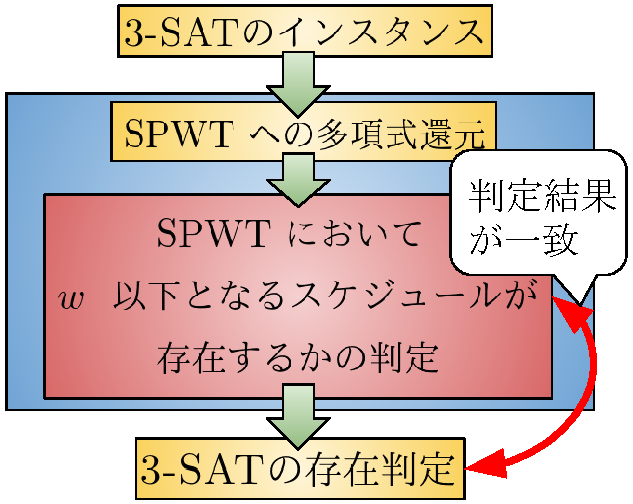
\includegraphics[width=5cm,bb=0 0 360 260
        ]{figure/reduction.pdf}
      \end{figure}
    \end{minipage}
  \end{tabular}
  \begin{block}{}
    本研究では以下が成立することを示す.
    \begin{enumerate}
      \item スケジュールにおける最大実行開始待ち時間が $w$ 以下であるかの判定が\alert{多項式時間}で可能である.
      \item 3 - SAT のインスタンスから 最大実行開始待ち時間最小化問題 のインスタンスが\alert{多項式時間}で構成可能であり,3 - SAT の判定結果と構成したインスタンスに対する $w$ 以下となるスケジュールの存在判定結果が\alert{一致}する.
    \end{enumerate}
  \end{block}
\end{frame}
%%%%%%%%%%%%%%%%%%%%%%%%%%%%%%%%%%%%%%%%%%%%%%%%%%%%%%%%%%%%%%%%%%%
\section{問題の分析}
\begin{frame}{問題の分析:既存のスケジューリング問題との対応}
  \begin{block}{既存のスケジューリング問題との共通部分}
    \begin{itemize}
      \item {$w = 0$ のとき,処理開始可能時刻ちょうどで処理を開始しなければならない.}
      \begin{itemize}
        \item {\alert{JIT ジョブスケジューリング問題}と対応する.}
      \end{itemize}
      \item {本研究で扱う問題は,処理開始可能時刻 と (処理開始可能時刻 + 処理時間 + $w$ )の区間で処理可能かという問題として捉えることができる.}
      \begin{itemize}
        \item {\alert{処理開始可能時刻と納期を持つスケジューリング問題}と対応する.}
      \end{itemize}
    \end{itemize}
  \end{block}
  \begin{block}{既存のスケジューリング問題との差分}
    \begin{itemize}
      \item {本研究で扱う問題は,納期 = 処理開始可能時刻 + 処理時間 + $w$ で表すことができる.}
      \begin{itemize}
        \item {処理開始可能時刻と納期を持つスケジューリング問題の\alert{部分問題}として捉えることができる.}
      \end{itemize}
    \end{itemize}
  \end{block}
\end{frame}
%%%%%%%%%%%%%%%%%%%%%%%%%%%%%%%%%%%%%%%%%%%%%%%%%%%%%%%%%%%%%%%%%%%
\section{研究成果}
\begin{frame}{研究成果}
  \begin{block}{研究成果}
    \begin{description}
      \item[成果 1:] 無関連並列機械モデルにおいて,機械数が入力の一部の場合,最大実行開始待ち時間最小化問題が NP 完全であることを明らかにした.
      \item[成果 2:] 同一並列機械モデルにおける最大実行開始待ち時間最小化問題に対して,ヒューリスティックの開発と解法に対する実験的評価を行った.
      \item[成果 3:] 分枝限定法の改良により分析対象を拡張することに成功した.
    \end{description}
  \end{block}
\end{frame}
%%%%%%%%%%%%%%%%%%%%%%%%%%%%%%%%%%%%%%%%%%%%%%%%%%%%%%%%%%%%%%%%%%%
\section{今後の課題}
\begin{frame}{今後の課題}

\end{frame}
%%%%%%%%%%%%%%%%%%%%%%%%%%%%%%%%%%%%%%%%%%%%%%%%%%%%%%%%%%%%%%%%%%%
\end{document}
